% Generated by `cer p17-tables`; do not edit. Coordinates are written from the artifacts.
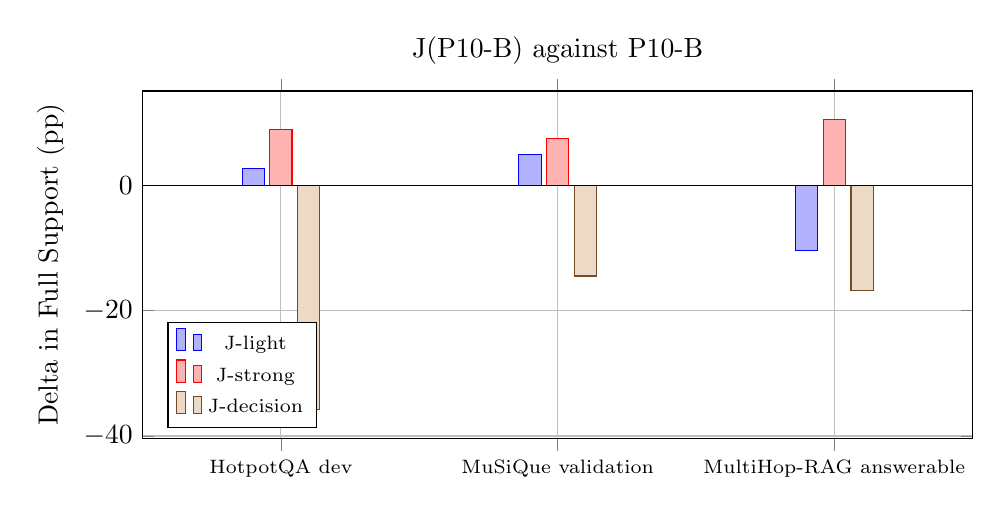
\begin{tikzpicture}
\begin{axis}[ybar, width=\columnwidth, height=6cm, bar width=8pt, enlarge x limits=0.25, xtick={0,1,2}, xticklabels={{HotpotQA dev},{MuSiQue validation},{MultiHop-RAG answerable}}, x tick label style={font=\scriptsize}, ylabel={Delta in Full Support (pp)}, grid=major, legend pos=south west, legend style={font=\scriptsize}, title={J(P10-B) against P10-B}]
\addplot coordinates {(0,2.62) (1,4.96) (2,-10.42)};
\addlegendentry{J-light}
\addplot coordinates {(0,8.94) (1,7.45) (2,10.42)};
\addlegendentry{J-strong}
\addplot coordinates {(0,-35.84) (1,-14.48) (2,-16.81)};
\addlegendentry{J-decision}
\draw (axis cs:-1,0) -- (axis cs:3,0);
\end{axis}
\end{tikzpicture}
